\documentclass[11pt,a4paper]{ctexart}
\usepackage[margin=2.35cm]{geometry}
\usepackage{amsmath,amssymb,booktabs,graphicx,hyperref,tikz,enumitem}
\usetikzlibrary{arrows.meta,positioning}
\hypersetup{colorlinks=true,linkcolor=black,urlcolor=blue}
\setlength{\parindent}{2em}
\setlength{\parskip}{0.25em}
\linespread{1.16}
\graphicspath{{../solution/results/}}

\title{人工智能第二次作业\\MNIST 手写数字识别实验报告}
\author{钟锦程\quad 2026210748\quad 电子工程系}
\date{2026 年秋}

\begin{document}
\maketitle
\begin{abstract}
我用 PyTorch 在 MNIST 上实现了线性分类器、几种全连接神经网络（MLP）和卷积神经网络（CNN）。线性模型用作加分项中的 baseline；MLP 比较隐藏层宽度与学习率；CNN 另外比较了训练时的轻量数据增强。训练集中的 6000 张图片专门作为验证集，模型选择只看验证准确率。最好的 MLP 在测试集上取得 97.75\% 的准确率，普通 CNN 为 98.88\%，增强 CNN 为 98.91\%。我还用固定旋转平移和自己生成的字体数字检查了模型遇到分布变化时的表现。
\end{abstract}
\setcounter{tocdepth}{1}
\tableofcontents
\newpage

\section{任务、环境与实验安排}
MNIST 中的每张图片是 $28\times28$ 的单通道灰度图，标签是 0 到 9 中的一个数字。模型读入图片后输出 10 个类别的分数，预测类别取分数最大的下标。完整数据包括 60000 张训练图片和 10000 张测试图片。

实验使用 macOS 26.6.2、Apple M5 Pro、24 GiB 内存、Python 3.11.15、PyTorch 2.14.1、torchvision 0.29.1。训练在 Apple MPS 上进行，绘图使用 Matplotlib 3.11.2。所有代码和运行方法位于\href{https://github.com/leo0302git/AI60240052/tree/main/assignment2/solution}{GitHub 项目的 assignment2/solution 目录}。

我把原始训练集按随机种子 2026 固定划分：54000 张用于更新参数，6000 张用于挑选模型；官方测试集的 10000 张只在训练结束后用于评估。线性模型、MLP 和 CNN 使用同一组下标与同样的标准测试集。这样在比较模型时，数据划分带来的差别会小一些。

\section{数据处理、训练与指标}
\subsection{从附件到模型输入}
程序优先从课程附件 \texttt{mnist.zip} 解压四个 IDX 文件；如果本地没有附件，可以通过 torchvision 下载 MNIST。像素原本是 0 到 255 的整数，我先除以 255 转成浮点数，再按训练数据常用的均值 0.1307 和标准差 0.3081 归一化：
\begin{equation}
z=\frac{x/255-0.1307}{0.3081}.
\end{equation}
这一步让输入的大部分数值靠近 0，便于神经网络训练。所有验证与标准测试图片都采用相同的处理。增强 CNN 只在训练图片上额外使用随机旋转（$\pm12^\circ$）和水平、竖直方向各至多 10\% 的平移。

\subsection{训练、验证和停止规则}
每次实验从固定随机种子开始初始化模型，用批大小 256 和 Adam 优化器，以交叉熵损失训练。默认最多训练 6 个 epoch。每轮结束后在验证集上计算准确率：若超过该实验此前的最好结果，就保存这一轮的权重；若连续两轮没有提高，就提前停止。最终测试使用保存的最好权重。MLP 的不同参数组合也只用验证准确率挑选。

\subsection{准确率与宏平均 F1}
准确率是预测正确的图片数除以总图片数。F1 需要先针对每个数字统计查准率与查全率：
\begin{equation}
P_c=\frac{TP_c}{TP_c+FP_c},\qquad
R_c=\frac{TP_c}{TP_c+FN_c},\qquad
F1_c=\frac{2P_cR_c}{P_c+R_c}.
\end{equation}
为了给十个数字同等权重，报告中的 F1 是 $\frac{1}{10}\sum_{c=0}^{9}F1_c$，即宏平均 F1。若某类没有预测样本，程序把相应分母保护为 1，其查准率视为 0。MNIST 的标签文件直接给出了类别整数；它与对 one-hot 标签取最大值所得到的类别一致。

\section{模型结构与作用}
下面的结构图由本实验按实际代码绘制。图中的数字表示张量尺寸，不包括批大小。

\subsection{线性分类器与 MLP}
线性分类器把 784 个像素直接映射到 10 个类别，参数数目为 $784\times10+10=7850$。它可以衡量加入隐藏层究竟带来了多少收益。

\begin{figure}[htbp]
\centering
\begin{tikzpicture}[node distance=0.28cm, box/.style={draw,rounded corners,align=center,font=\small,minimum height=0.9cm,inner sep=4pt}, >={Latex[length=2mm]}]
\node[box] (i) {输入图片\\$1\times28\times28$};
\node[box,right=of i] (f) {展平\\784};
\node[box,right=of f] (h) {全连接\\$784\to256$};
\node[box,right=of h] (r) {ReLU\\Dropout 0.2};
\node[box,right=of r] (o) {全连接\\$256\to10$};
\draw[->] (i)--(f); \draw[->] (f)--(h); \draw[->] (h)--(r); \draw[->] (r)--(o);
\end{tikzpicture}
\caption{自己绘制的 MLP 结构图；线性 baseline 省去中间的隐藏层与激活层。}
\end{figure}

MLP 的隐藏层先组合像素信息，ReLU 提供非线性能力，Dropout 在训练时随机舍弃 20\% 的隐藏单元，最后一层输出 10 个类别分数。上图使用宽度 256，对应 203530 个参数；比较实验还将隐藏层宽度改为 128。

\subsection{CNN}
CNN 保留图片的二维邻近关系。第一个 $3\times3$ 卷积产生 16 张特征图；池化将宽高减半。第二个卷积产生 32 张特征图，再池化到 $7\times7$，最后由全连接层完成分类。两个 CNN 的结构和参数量完全相同，区别只在训练时是否增强图片。

\begin{figure}[htbp]
\centering
\begin{tikzpicture}[node distance=0.22cm, box/.style={draw,rounded corners,align=center,font=\footnotesize,minimum height=0.95cm,inner sep=3pt}, >={Latex[length=2mm]}]
\node[box] (i) {图片\\$1\times28\times28$};
\node[box,right=of i] (c1) {卷积 $3\times3$ + ReLU\\$16\times28\times28$};
\node[box,right=of c1] (p1) {池化 $2\times2$\\$16\times14\times14$};
\node[box,right=of p1] (c2) {卷积 $3\times3$ + ReLU\\$32\times14\times14$};
\node[box,right=of c2] (p2) {池化 $2\times2$\\$32\times7\times7$};
\draw[->] (i)--(c1); \draw[->] (c1)--(p1); \draw[->] (p1)--(c2); \draw[->] (c2)--(p2);
\end{tikzpicture}

\vspace{0.35em}
$32\times7\times7\xrightarrow{\text{展平}}1568
\xrightarrow{\text{全连接 + ReLU}}128
\xrightarrow{\text{Dropout 0.2 + 全连接}}10$
\caption{自己绘制的 CNN 结构图。卷积核提取局部形状，池化缩小特征图，末端输出类别分数。}
\end{figure}

CNN 共 206922 个可学习参数，与宽度 256 的 MLP 接近。因此二者的比较也有一定参考价值：参数数量相近时，利用图像空间结构的方式会影响识别效果。

\section{结果与参数对比}
\subsection{标准测试集}
表 \ref{tab:main} 列出六次实际训练的结果。时间包含各 epoch 的训练、验证与最佳权重保存，不含首次解压数据和额外测试。百分数均由程序记录的原始小数换算而来。

\begin{table}[htbp]
\centering\small
\caption{MNIST 实验结果；所有模型均按验证集最佳权重测试。}\label{tab:main}
\begin{tabular}{lrrrrr}
\toprule
模型 & 参数量 & 最佳验证准确率 & 测试准确率 & 测试宏 F1 & 训练秒数\\
\midrule
线性 baseline & 7850 & 91.18\% & 92.22\% & 92.11\% & 8.70\\
MLP，宽度 128 & 101770 & 97.07\% & 97.53\% & 97.51\% & 8.85\\
MLP，宽度 256 & 203530 & 97.50\% & 97.75\% & 97.73\% & 8.97\\
MLP，宽度 256，低学习率 & 203530 & 96.05\% & 96.70\% & 96.67\% & 8.79\\
普通 CNN & 206922 & 98.75\% & 98.88\% & 98.87\% & 12.35\\
增强 CNN & 206922 & 98.55\% & 98.91\% & 98.91\% & 15.66\\
\bottomrule
\end{tabular}
\end{table}

我首先把 MLP 宽度从 128 增至 256，学习率均为 0.001。验证准确率从 97.07\% 升至 97.50\%，所以后者被选为本实验的 MLP。保持宽度 256、把学习率改为 0.0003 后，在同样最多 6 轮的训练预算下验证准确率降至 96.05\%。学习率变小使每步更新幅度变小，这组设置在 6 轮内还没有达到原设置的水平；我没有据此判断低学习率在更长训练中一定更差。

图 \ref{fig:curves} 显示每轮验证准确率和训练损失。普通 CNN 比 MLP 更早达到高准确率，线性模型则较早出现平台期。普通 CNN 和增强 CNN 在标准测试上的准确率只相差 0.03 个百分点，这个小差别不足以说明增强显著提高了原始测试集表现。

\begin{figure}[htbp]
\centering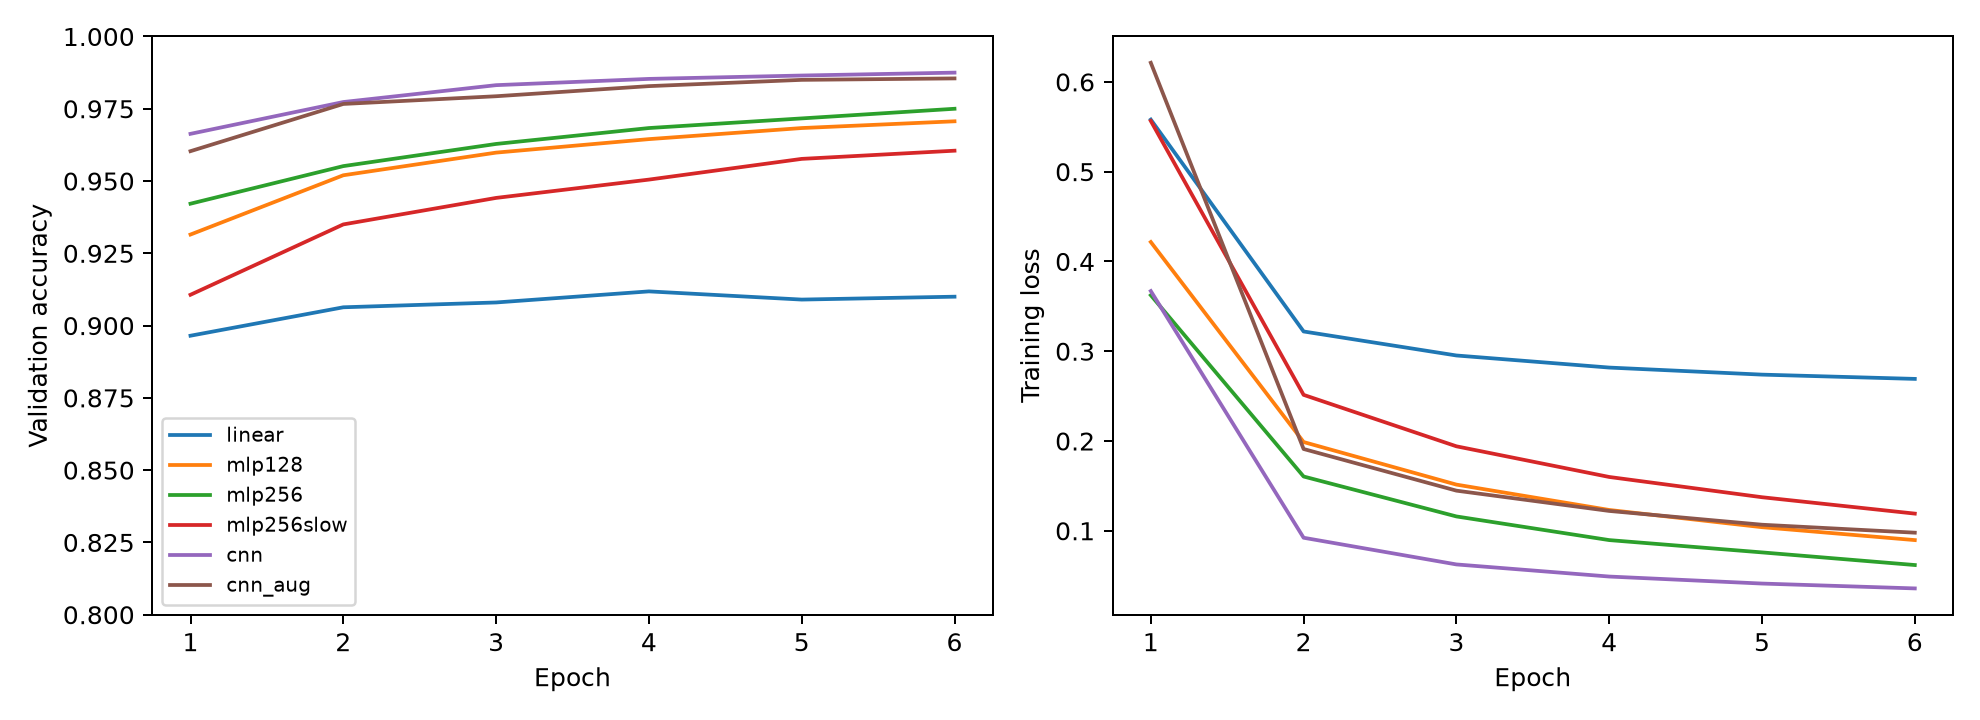
\includegraphics[width=0.95\linewidth]{learning_curves.png}
\caption{六组实验的逐轮验证准确率和训练损失，由本实验代码绘制。}\label{fig:curves}
\end{figure}

\subsection{混淆情况}
图 \ref{fig:confusion} 是增强 CNN 在标准测试集上的混淆矩阵。对角线越深，说明相应数字识别正确的数量越多。10000 张图片中有 9891 张被正确分类。较多的单向错误包括真实数字 7 被预测成 9（6 张）和真实数字 2 被预测成 0（6 张）。这些都只是少量样本，仍说明形状相近的数字可能出现歧义。

\begin{figure}[htbp]
\centering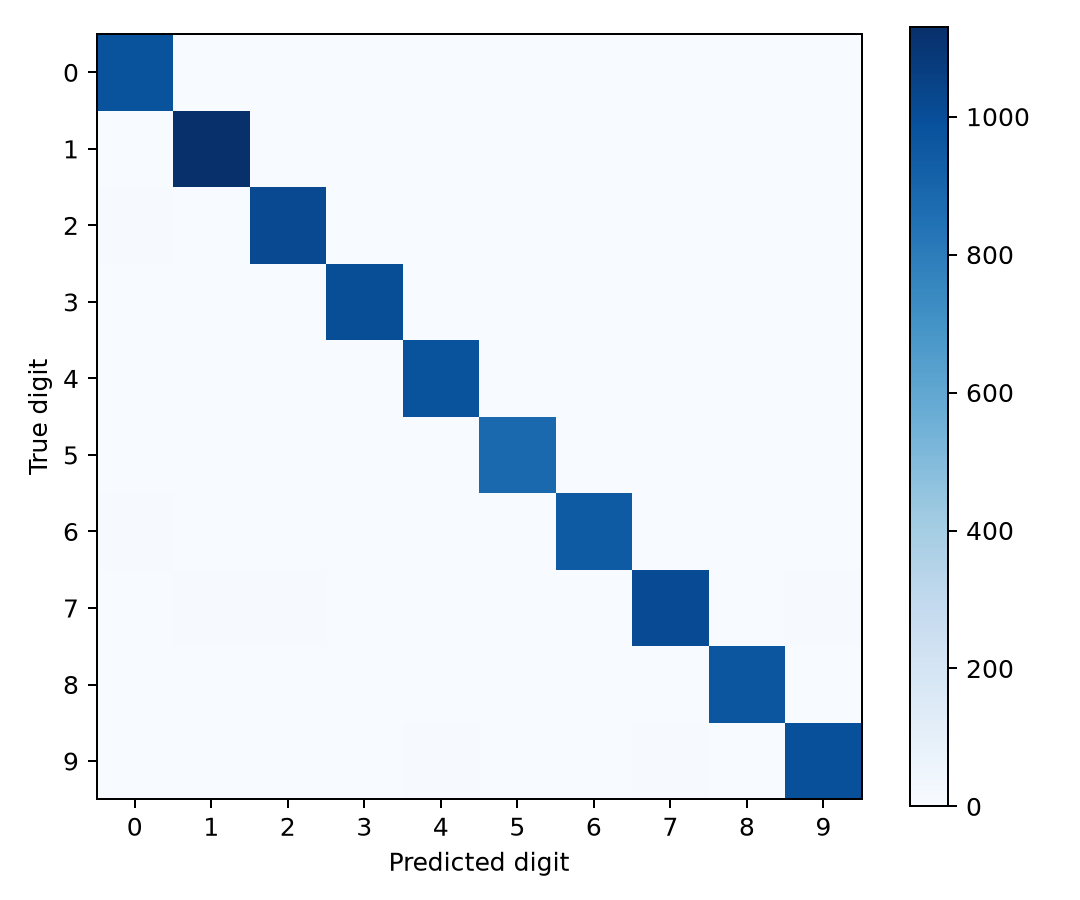
\includegraphics[width=0.64\linewidth]{confusion_matrix.png}
\caption{增强 CNN 的 MNIST 测试集混淆矩阵，纵轴是真实类别，横轴是预测类别。}\label{fig:confusion}
\end{figure}

\section{额外 baseline、数据增强和鲁棒性}
线性分类器是加分实验中的额外 baseline。它的测试准确率达到 92.22\%，说明很多数字仅凭像素位置也能区分；但与 MLP 的 97.75\% 和 CNN 的 98.88\% 相比，线性映射处理笔画变化的能力有限。

为了观察更困难的输入，我构造了两组补充测试。第一组对官方测试集每张图片固定旋转 $15^\circ$ 并平移 $(2,-2)$ 像素，共 10000 张。第二组用 Matplotlib 附带的三种 DejaVu 字体，每个数字在三个横向位置生成一张 $28\times28$ 灰度图，共 $3\times10\times3=90$ 张。它们是我自己生成的印刷体图片，和真实的手写照片不同；图 \ref{fig:font} 展示了其中每个数字的一张。

\begin{figure}[htbp]
\centering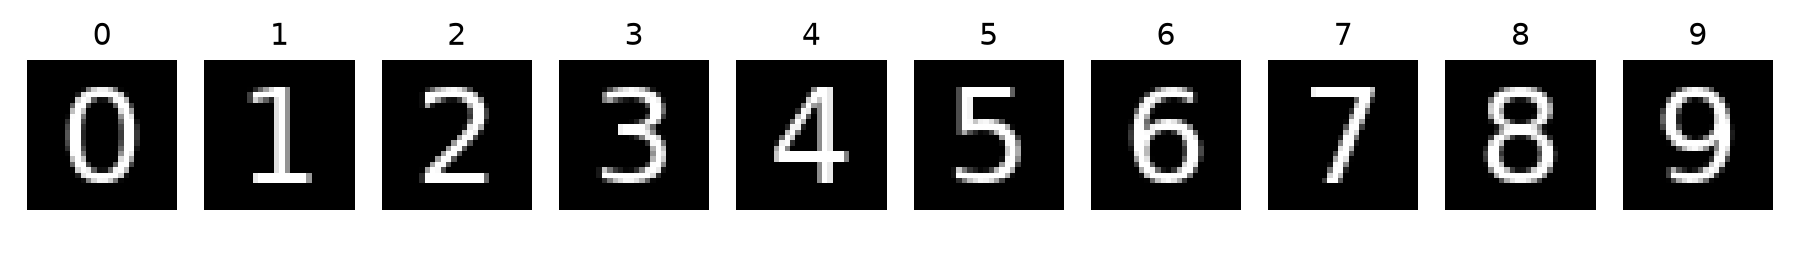
\includegraphics[width=0.95\linewidth]{font_digits.png}
\caption{自制字体数字示例，每列是一类数字。}\label{fig:font}
\end{figure}

\begin{table}[htbp]
\centering
\caption{同一最佳权重在三组测试图片上的准确率。}\label{tab:robust}
\begin{tabular}{lrrr}
\toprule
模型 & 原始 MNIST（10000） & 固定旋转平移（10000） & 字体数字（90）\\
\midrule
线性 baseline & 92.22\% & 41.32\% & 51.11\%\\
最佳 MLP & 97.75\% & 66.35\% & 74.44\%\\
普通 CNN & 98.88\% & 82.68\% & 85.56\%\\
增强 CNN & 98.91\% & 95.73\% & 98.89\%\\
\bottomrule
\end{tabular}
\end{table}

增强 CNN 在固定旋转平移测试上比普通 CNN 高 13.05 个百分点，在字体数字上高 13.33 个百分点。训练时见过多种角度和位置的数字，可能使模型减少对某一个固定笔画位置的依赖。字体测试只有 90 张，而且字体种类有限，所以这个结果只能说明模型对这组自制图片适应较好，不能代替更多真实手写图片的评估。

\section{问题与思考}
\subsection{什么时候停止训练？}
我设置最多 6 个 epoch，并保存验证准确率最高的一轮。若连续两轮没有刷新最高值，就提前停止。六组正式实验都在第 6 轮结束，其中线性分类器的最佳权重来自第 4 轮。由此可见，最后一轮的参数不一定就是最好的。

固定训练轮数容易安排时间，也方便不同实验在同一预算下比较。但不同模型收敛速度不同，固定轮数可能使某个模型训练不足，也可能使已经达到最佳验证效果的模型继续拟合训练集。验证集规则可以自动选权重并减少多余训练；它同时需要额外数据和每轮验证时间，若反复尝试很多参数，也可能逐渐对这一份验证集过度适应。因此我的参数搜索保持在较少的三组 MLP 设置。

\subsection{参数怎样初始化？}
本实验没有手动改写 PyTorch 的层初始化：\texttt{Linear} 和 \texttt{Conv2d} 的默认权重使用与输入连接数相关的 Kaiming uniform 初始化，偏置使用相应范围的均匀分布。固定随机种子使同一种结构的初始随机状态可重复。初始值需要有一定随机性；若同一层所有权重都设成零，同层神经元接收相同梯度，难以学出不同特征。

零均值高斯初始化可让权重围绕 0 分布，但方差要结合层的输入、输出规模选择，过大可能使激活值变得很大，过小则可能让信号逐层衰减。ReLU 网络常用 He/Kaiming 初始化来照顾其只保留正半轴的特点；tanh 一类对称激活常用 Xavier 初始化。正交初始化让权重矩阵在若干方向上保持较独立的尺度，较深网络或循环网络中有价值。偏置通常可以初始化为零，因为权重已经打破了神经元之间的对称性。

\subsection{怎样减少过拟合？}
过拟合时，训练集继续变好，但验证集停滞甚至下降。我在 MLP 和 CNN 的全连接部分使用 0.2 的 Dropout，在增强 CNN 上对训练图片随机旋转和平移，还根据验证准确率挑选最佳权重。这三种方法分别减少对少数隐藏单元、固定图像位置和最后一轮参数的依赖。也可以尝试权重衰减、收集更多训练图片或缩小模型，但应查看验证集的变化再决定。本实验 CNN 第 6 轮训练准确率约 98.90\%，验证准确率约 98.75\%，没有出现很大的差距；继续训练时仍需关注这一差距是否扩大。

\subsection{各模型有什么优缺点？}
线性 baseline 只有 7850 个参数，结构容易理解，训练也快，但只能做一次线性映射。MLP 通过 ReLU 和隐藏层组合像素信息，本实验从线性模型的 92.22\% 提升到 97.75\%；展平图片后，它仍需从数据中学习图像邻近位置之间的关系。CNN 的局部卷积核和池化更适合数字笔画，参数量与最佳 MLP 接近时准确率达到 98.88\%。它的计算过程稍复杂，训练时间也更长。增强 CNN 训练更慢、原始测试提升很小，但在本实验构造的位置变化和字体数字上表现更稳定。

\subsection{换一批图片还可靠吗？}
表 \ref{tab:robust} 已经给出了两组补充测试。普通 CNN 在原始 MNIST 上是 98.88\%，遇到固定旋转平移时降到 82.68\%；这说明一个高标准测试分数不能单独说明模型能处理所有写法。增强 CNN 在该组上达到 95.73\%，对这类已在训练中模拟过的变化适应更好。90 张字体图片给了另一个角度，但它们是印刷体，不是个人手写照片。下一步可以收集不同人用手机拍摄的真实数字，检查背景、笔画粗细和居中处理造成的影响。

\section{心得与不足}
这个实验让我把数据划分、模型选择和最终评估串起来理解了。开始时我只关注模型的准确率，后来发现验证集的用途同样重要：如果用测试集挑参数，最后的测试分数就难以代表未见数据的效果。线性模型、MLP 和 CNN 的逐步比较，也让我更直观地看到图像结构信息的作用。

目前只试了少量超参数，六轮预算也偏短；在字体图片上的结果不能代表真实手写照片。我保留了固定随机种子、全部实验记录和一条可运行命令，今后可以在相同划分上继续检查更多真实图片与其他增强方式。

\end{document}
